\chapter{Evaluation}

\section{Dieharder Results}

Dieharder is designed to push the tests to unambiguous failure CITE Robert G. Brown's General Tools Page (duke.edu) . It contains a number of flag options to alter the parameters of the tests and change their acceptance criteria. The command used to run the Dieharder test suite for this project was:\newline

Dieharder -a -k 2 -Y 1 -f <filename>\newline

The -a flag runs all the tests in the dieharder test suite, as described in  section BLANK. The -k flag is the ks-flag K sminorv thing. The -Y flag is the Xtrategy flag which is used to control the ‘test to failure’ modes. CITE  rgb. This flag is set to 1 to use the ‘resolve ambiguity’ mode. Dieharder can return ‘weak’ as a test result which can be difficult to interpret. Even perfect random numbers will return some ‘weak’ results at some point because the p-values are uniformly distributed and will have a result in the tails of the distribution from time to time. Even if a test returns more than one weak result, this is not conclusive evidence that the data is non-random. The ‘resolve ambiguity’ mode resolves this issue by adding p-samples (in blocks of 100) until the test results in a definitive pass, weak or it proceeds to failure. \newline

\subsection{TEKs Results}
Table for teks
\begin{longtable}{cccccc}
\toprule
Test Name & $n$ & $N$ & $d$ & $p$-value & Result \\
\midrule
diehard\_birthdays & 0 & 100 & 100 & 0.98740819 & PASSED \\
diehard\_operm5 & 0 & 1000000 & 100 & 0.95452336 & PASSED \\
diehard\_rank\_32x32 & 0 & 40000 & 100 & 0.59831249 & PASSED \\
diehard\_rank\_6x8 & 0 & 100000 & 100 & 0.54719972 & PASSED \\
diehard\_bitstream & 0 & 2097152 & 100 & 0.38293106 & PASSED \\
diehard\_opso & 0 & 2097152 & 100 & 0.35772252 & PASSED \\
diehard\_oqso & 0 & 2097152 & 100 & 0.69390124 & PASSED \\
diehard\_dna & 0 & 2097152 & 100 & 0.42865960 & PASSED \\
diehard\_count\_1s\_str & 0 & 256000 & 100 & 0.29872959 & PASSED \\
diehard\_count\_1s\_byt & 0 & 256000 & 100 & 0.08174702 & PASSED \\
diehard\_parking\_lot & 0 & 12000 & 100 & 0.91403506 & PASSED \\
diehard\_2dsphere & 2 & 8000 & 100 & 0.23586557 & PASSED \\
diehard\_3dsphere & 3 & 4000 & 100 & 0.63468855 & PASSED \\
diehard\_squeeze & 0 & 100000 & 100 & 0.28961226 & PASSED \\
diehard\_sums & 0 & 100 & 100 & 0.00750044 & PASSED \\
diehard\_runs & 0 & 100000 & 100 & 0.88654068 & PASSED \\
diehard\_runs & 0 & 100000 & 100 & 0.23670757 & PASSED \\
diehard\_craps & 0 & 200000 & 100 & 0.89199102 & PASSED \\
diehard\_craps & 0 & 200000 & 100 & 0.68235234 & PASSED \\
marsaglia\_tsang\_gcd & 0 & 10000000 & 100 & 0.03007484 & PASSED \\
marsaglia\_tsang\_gcd & 0 & 10000000 & 100 & 0.32230404 & PASSED \\
sts\_monobit & 1 & 100000 & 100 & 0.15180696 & PASSED \\
sts\_runs & 2 & 100000 & 100 & 0.50053774 & PASSED \\
sts\_serial & 1 & 100000 & 100 & 0.05380206 & PASSED \\
sts\_serial & 2 & 100000 & 100 & 0.84490409 & PASSED \\
sts\_serial & 3 & 100000 & 100 & 0.39453536 & PASSED \\
sts\_serial & 3 & 100000 & 100 & 0.12475855 & PASSED \\
sts\_serial & 4 & 100000 & 100 & 0.01782397 & PASSED \\
sts\_serial & 4 & 100000 & 100 & 0.62109194 & PASSED \\
sts\_serial & 5 & 100000 & 100 & 0.46912814 & PASSED \\
sts\_serial & 5 & 100000 & 100 & 0.77530843 & PASSED \\
sts\_serial & 6 & 100000 & 100 & 0.29587704 & PASSED \\
sts\_serial & 6 & 100000 & 100 & 0.56715645 & PASSED \\
sts\_serial & 7 & 100000 & 100 & 0.84905787 & PASSED \\
sts\_serial & 7 & 100000 & 100 & 0.40116976 & PASSED \\
sts\_serial & 8 & 100000 & 100 & 0.93664924 & PASSED \\
sts\_serial & 8 & 100000 & 100 & 0.10486711 & PASSED \\
sts\_serial & 9 & 100000 & 100 & 0.16044494 & PASSED \\
sts\_serial & 9 & 100000 & 100 & 0.05301976 & PASSED \\
sts\_serial & 10 & 100000 & 100 & 0.92312992 & PASSED \\
sts\_serial & 10 & 100000 & 100 & 0.35673434 & PASSED \\
sts\_serial & 11 & 100000 & 100 & 0.98426112 & PASSED \\
sts\_serial & 11 & 100000 & 100 & 0.80067302 & PASSED \\
sts\_serial & 12 & 100000 & 100 & 0.99373847 & PASSED \\
sts\_serial & 12 & 100000 & 100 & 0.88803021 & PASSED \\
sts\_serial & 13 & 100000 & 100 & 0.66824428 & PASSED \\
sts\_serial & 13 & 100000 & 100 & 0.50746190 & PASSED \\
sts\_serial & 14 & 100000 & 100 & 0.98238726 & PASSED \\
sts\_serial & 14 & 100000 & 100 & 0.26538675 & PASSED \\
sts\_serial & 15 & 100000 & 100 & 0.39728743 & PASSED \\
sts\_serial & 15 & 100000 & 100 & 0.97041422 & PASSED \\
sts\_serial & 16 & 100000 & 100 & 0.25630622 & PASSED \\
sts\_serial & 16 & 100000 & 100 & 0.05364901 & PASSED \\
rgb\_bitdist & 1 & 100000 & 100 & 0.44512215 & PASSED \\
rgb\_bitdist & 2 & 100000 & 100 & 0.23502241 & PASSED \\
rgb\_bitdist & 3 & 100000 & 100 & 0.32191988 & PASSED \\
rgb\_bitdist & 4 & 100000 & 100 & 0.22761597 & PASSED \\
rgb\_bitdist & 5 & 100000 & 100 & 0.30123524 & PASSED \\
rgb\_bitdist & 6 & 100000 & 100 & 0.83677612 & PASSED \\
rgb\_bitdist & 7 & 100000 & 100 & 0.68327297 & PASSED \\
rgb\_bitdist & 8 & 100000 & 100 & 0.91556750 & PASSED \\
rgb\_bitdist & 9 & 100000 & 100 & 0.98795982 & PASSED \\
rgb\_bitdist & 10 & 100000 & 100 & 0.19379581 & PASSED \\
rgb\_bitdist & 11 & 100000 & 100 & 0.53441056 & PASSED \\
rgb\_bitdist & 12 & 100000 & 100 & 0.64656408 & PASSED \\
rgb\_minimum\_distance & 2 & 10000 & 1000 & 0.95411695 & PASSED \\
rgb\_minimum\_distance & 3 & 10000 & 1000 & 0.54118074 & PASSED \\
rgb\_minimum\_distance & 4 & 10000 & 1000 & 0.25746852 & PASSED \\
rgb\_minimum\_distance & 5 & 10000 & 1000 & 0.52797286 & PASSED \\
rgb\_permutations & 2 & 100000 & 100 & 0.68240647 & PASSED \\
rgb\_permutations & 3 & 100000 & 100 & 0.71482801 & PASSED \\
rgb\_permutations & 4 & 100000 & 100 & 0.95248263 & PASSED \\
rgb\_permutations & 5 & 100000 & 100 & 0.76625613 & PASSED \\
rgb\_lagged\_sum & 0 & 1000000 & 100 & 0.86229846 & PASSED \\
rgb\_lagged\_sum & 1 & 1000000 & 100 & 0.85446006 & PASSED \\
rgb\_lagged\_sum & 2 & 1000000 & 100 & 0.72559541 & PASSED \\
rgb\_lagged\_sum & 3 & 1000000 & 100 & 0.44885925 & PASSED \\
rgb\_lagged\_sum & 4 & 1000000 & 100 & 0.96344825 & PASSED \\
rgb\_lagged\_sum & 5 & 1000000 & 100 & 0.25164161 & PASSED \\
rgb\_lagged\_sum & 6 & 1000000 & 100 & 0.28999845 & PASSED \\
rgb\_lagged\_sum & 7 & 1000000 & 100 & 0.25609882 & PASSED \\
rgb\_lagged\_sum & 8 & 1000000 & 100 & 0.29886696 & PASSED \\
rgb\_lagged\_sum & 9 & 1000000 & 100 & 0.63708913 & PASSED \\
rgb\_lagged\_sum & 10 & 1000000 & 100 & 0.11998965 & PASSED \\
rgb\_lagged\_sum & 11 & 1000000 & 100 & 0.02340253 & PASSED \\
rgb\_lagged\_sum & 12 & 1000000 & 100 & 0.92961604 & PASSED \\
rgb\_lagged\_sum & 13 & 1000000 & 100 & 0.53433063 & PASSED \\
rgb\_lagged\_sum & 14 & 1000000 & 100 & 0.63635183 & PASSED \\
rgb\_lagged\_sum & 15 & 1000000 & 100 & 0.12766584 & PASSED \\
rgb\_lagged\_sum & 16 & 1000000 & 100 & 0.35077156 & PASSED \\
rgb\_lagged\_sum & 17 & 1000000 & 100 & 0.75718004 & PASSED \\
rgb\_lagged\_sum & 18 & 1000000 & 100 & 0.35537855 & PASSED \\
rgb\_lagged\_sum & 19 & 1000000 & 100 & 0.73789139 & PASSED \\
rgb\_lagged\_sum & 20 & 1000000 & 100 & 0.14002184 & PASSED \\
rgb\_lagged\_sum & 21 & 1000000 & 100 & 0.05885242 & PASSED \\
rgb\_lagged\_sum & 22 & 1000000 & 100 & 0.34112889 & PASSED \\
rgb\_lagged\_sum & 23 & 1000000 & 100 & 0.92939060 & PASSED \\
rgb\_lagged\_sum & 24 & 1000000 & 100 & 0.41104728 & PASSED \\
rgb\_lagged\_sum & 25 & 1000000 & 100 & 0.68323308 & PASSED \\
rgb\_lagged\_sum & 26 & 1000000 & 100 & 0.07730139 & PASSED \\
rgb\_lagged\_sum & 27 & 1000000 & 100 & 0.07269523 & PASSED \\
rgb\_lagged\_sum & 28 & 1000000 & 100 & 0.23320287 & PASSED \\
rgb\_lagged\_sum & 29 & 1000000 & 100 & 0.36469854 & PASSED \\
rgb\_lagged\_sum & 30 & 1000000 & 100 & 0.21883650 & PASSED \\
rgb\_lagged\_sum & 31 & 1000000 & 100 & 0.33511740 & PASSED \\
rgb\_lagged\_sum & 32 & 1000000 & 100 & 0.05785507 & PASSED \\
rgb\_kstest\_test & 0 & 10000 & 1000 & 0.65613857 & PASSED \\
dab\_bytedistrib & 0 & 51200000 & 1 & 0.60605570 & PASSED \\
dab\_dct & 256 & 50000 & 1 & 0.49995832 & PASSED \\
dab\_filltree & 32 & 15000000 & 1 & 0.75555153 & PASSED \\
dab\_filltree & 32 & 15000000 & 1 & 0.40968822 & PASSED \\
dab\_filltree2 & 0 & 5000000 & 1 & 0.10438267 & PASSED \\
dab\_filltree2 & 1 & 5000000 & 1 & 0.80708126 & PASSED \\
dab\_monobit2 & 12 & 65000000 & 1 & 0.74779198 & PASSED \\
\bottomrule
\caption{Dieharder Results of TEKS.}
\label{table}
\end{longtable}

\subsection{Random keys Results}
Table for random value
\begin{longtable}{cccccc}
\toprule
Test Name & $n$ & $N$ & $d$ & $p$-value & Result \\
\midrule
\endhead
diehard\_birthdays & 0 & 100 & 100 & 0.76394892 & PASSED \\
diehard\_operm5 & 0 & 1000000 & 100 & 0.18935905 & PASSED \\
diehard\_rank\_32x32 & 0 & 40000 & 100 & 0.21580801 & PASSED \\
diehard\_rank\_6x8 & 0 & 100000 & 100 & 0.02770416 & PASSED \\
diehard\_bitstream & 0 & 2097152 & 100 & 0.75370418 & PASSED \\
diehard\_opso & 0 & 2097152 & 100 & 0.32644238 & PASSED \\
diehard\_oqso & 0 & 2097152 & 100 & 0.89648137 & PASSED \\
diehard\_dna & 0 & 2097152 & 100 & 0.59449638 & PASSED \\
diehard\_count\_1s\_str & 0 & 256000 & 100 & 0.37707042 & PASSED \\
diehard\_count\_1s\_byt & 0 & 256000 & 100 & 0.38613176 & PASSED \\
diehard\_parking\_lot & 0 & 12000 & 100 & 0.98428899 & PASSED \\
diehard\_2dsphere & 2 & 8000 & 100 & 0.57449647 & PASSED \\
diehard\_3dsphere & 3 & 4000 & 100 & 0.47967697 & PASSED \\
diehard\_squeeze & 0 & 100000 & 100 & 0.02908390 & PASSED \\
diehard\_sums & 0 & 100 & 100 & 0.01302183 & PASSED \\
diehard\_runs & 0 & 100000 & 100 & 0.21268023 & PASSED \\
diehard\_runs & 0 & 100000 & 100 & 0.48718248 & PASSED \\
diehard\_craps & 0 & 200000 & 100 & 0.43589180 & PASSED \\
diehard\_craps & 0 & 200000 & 100 & 0.48427891 & PASSED \\
marsaglia\_tsang\_gcd & 0 & 10000000 & 100 & 0.39544378 & PASSED \\
marsaglia\_tsang\_gcd & 0 & 10000000 & 100 & 0.00073901 & WEAK \\
marsaglia\_tsang\_gcd & 0 & 10000000 & 200 & 0.20103622 & PASSED \\
marsaglia\_tsang\_gcd & 0 & 10000000 & 200 & 0.00000116 & WEAK \\
marsaglia\_tsang\_gcd & 0 & 10000000 & 300 & 0.15296148 & PASSED \\
marsaglia\_tsang\_gcd & 0 & 10000000 & 300 & 0.00000000 & FAILED \\
sts\_monobit & 1 & 100000 & 100 & 0.46954912 & PASSED \\
sts\_runs & 2 & 100000 & 100 & 0.99997882 & WEAK \\
sts\_runs & 2 & 100000 & 200 & 0.65262205 & PASSED \\
sts\_serial & 1 & 100000 & 100 & 0.75039800 & PASSED \\
sts\_serial & 2 & 100000 & 100 & 0.46782328 & PASSED \\
sts\_serial & 3 & 100000 & 100 & 0.96422500 & PASSED \\
sts\_serial & 3 & 100000 & 100 & 0.38336381 & PASSED \\
sts\_serial & 4 & 100000 & 100 & 0.78436629 & PASSED \\
sts\_serial & 4 & 100000 & 100 & 0.32790423 & PASSED \\
sts\_serial & 5 & 100000 & 100 & 0.93561180 & PASSED \\
sts\_serial & 5 & 100000 & 100 & 0.78894832 & PASSED \\
sts\_serial & 6 & 100000 & 100 & 0.30162394 & PASSED \\
sts\_serial & 6 & 100000 & 100 & 0.45041009 & PASSED \\
sts\_serial & 7 & 100000 & 100 & 0.60514729 & PASSED \\
sts\_serial & 7 & 100000 & 100 & 0.52470608 & PASSED \\
sts\_serial & 8 & 100000 & 100 & 0.38468429 & PASSED \\
sts\_serial & 8 & 100000 & 100 & 0.97346520 & PASSED \\
sts\_serial & 9 & 100000 & 100 & 0.67677659 & PASSED \\
sts\_serial & 9 & 100000 & 100 & 0.21257824 & PASSED \\
sts\_serial & 10 & 100000 & 100 & 0.06065198 & PASSED \\
sts\_serial & 10 & 100000 & 100 & 0.19676120 & PASSED \\
sts\_serial & 11 & 100000 & 100 & 0.25074198 & PASSED \\
sts\_serial & 11 & 100000 & 100 & 0.44324414 & PASSED \\
sts\_serial & 12 & 100000 & 100 & 0.06981655 & PASSED \\
sts\_serial & 12 & 100000 & 100 & 0.26688079 & PASSED \\
sts\_serial & 13 & 100000 & 100 & 0.50138141 & PASSED \\
sts\_serial & 13 & 100000 & 100 & 0.51148391 & PASSED \\
sts\_serial & 14 & 100000 & 100 & 0.38406027 & PASSED \\
sts\_serial & 14 & 100000 & 100 & 0.32968726 & PASSED \\
sts\_serial & 15 & 100000 & 100 & 0.20468696 & PASSED \\
sts\_serial & 15 & 100000 & 100 & 0.21397465 & PASSED \\
sts\_serial & 16 & 100000 & 100 & 0.16604967 & PASSED \\
sts\_serial & 16 & 100000 & 100 & 0.60748515 & PASSED \\
rgb\_bitdist & 1 & 100000 & 100 & 0.36452077 & PASSED \\
rgb\_bitdist & 2 & 100000 & 100 & 0.94306987 & PASSED \\
rgb\_bitdist & 3 & 100000 & 100 & 0.80290189 & PASSED \\
rgb\_bitdist & 4 & 100000 & 100 & 0.29185388 & PASSED \\
rgb\_bitdist & 5 & 100000 & 100 & 0.69257767 & PASSED \\
rgb\_bitdist & 6 & 100000 & 100 & 0.95139967 & PASSED \\
rgb\_bitdist & 7 & 100000 & 100 & 0.57919220 & PASSED \\
rgb\_bitdist & 8 & 100000 & 100 & 0.45468153 & PASSED \\
rgb\_bitdist & 9 & 100000 & 100 & 0.14850293 & PASSED \\
rgb\_bitdist & 10 & 100000 & 100 & 0.54937469 & PASSED \\
rgb\_bitdist & 11 & 100000 & 100 & 0.28545144 & PASSED \\
rgb\_bitdist & 12 & 100000 & 100 & 0.99636354 & WEAK \\
rgb\_bitdist & 12 & 100000 & 200 & 0.29765398 & PASSED \\
rgb\_minimum\_distance & 2 & 10000 & 1000 & 0.99960225 & WEAK \\
rgb\_minimum\_distance & 2 & 10000 & 1100 & 0.99544792 & WEAK \\
rgb\_minimum\_distance & 2 & 10000 & 1200 & 0.99960423 & WEAK \\
rgb\_minimum\_distance & 2 & 10000 & 1300 & 0.76490064 & PASSED \\
rgb\_minimum\_distance & 3 & 10000 & 1000 & 0.88490597 & PASSED \\
rgb\_minimum\_distance & 4 & 10000 & 1000 & 0.56548230 & PASSED \\
rgb\_minimum\_distance & 5 & 10000 & 1000 & 0.84433241 & PASSED \\
rgb\_permutations & 2 & 100000 & 100 & 0.81514673 & PASSED \\
rgb\_permutations & 3 & 100000 & 100 & 0.86382468 & PASSED \\
rgb\_permutations & 4 & 100000 & 100 & 0.99152004 & PASSED \\
rgb\_permutations & 4 & 100000 & 100 & 0.99152004 & PASSED \\
rgb\_permutations & 5 & 100000 & 100 & 0.31316379 & PASSED \\
rgb\_lagged\_sum & 0 & 1000000 & 100 & 0.26035279 & PASSED \\
rgb\_lagged\_sum & 1 & 1000000 & 100 & 0.99920642 & WEAK \\
rgb\_lagged\_sum & 1 & 1000000 & 200 & 0.29519499 & PASSED \\
rgb\_lagged\_sum & 2 & 1000000 & 100 & 0.28259248 & PASSED \\
rgb\_lagged\_sum & 3 & 1000000 & 100 & 0.99684866 & WEAK \\
rgb\_lagged\_sum & 3 & 1000000 & 200 & 0.75546305 & PASSED \\
rgb\_lagged\_sum & 4 & 1000000 & 100 & 0.97658438 & PASSED \\
rgb\_lagged\_sum & 5 & 1000000 & 100 & 0.44382799 & PASSED \\
rgb\_lagged\_sum & 6 & 1000000 & 100 & 0.97652946 & PASSED \\
rgb\_lagged\_sum & 7 & 1000000 & 100 & 0.87715734 & PASSED \\
rgb\_lagged\_sum & 8 & 1000000 & 100 & 0.42657999 & PASSED \\
rgb\_lagged\_sum & 9 & 1000000 & 100 & 0.32151735 & PASSED \\
rgb\_lagged\_sum & 10 & 1000000 & 100 & 0.48476972 & PASSED \\
rgb\_lagged\_sum & 11 & 1000000 & 100 & 0.94092042 & PASSED \\
rgb\_lagged\_sum & 12 & 1000000 & 100 & 0.72099398 & PASSED \\
rgb\_lagged\_sum & 13 & 1000000 & 100 & 0.81002140 & PASSED \\
rgb\_lagged\_sum & 14 & 1000000 & 100 & 0.15611012 & PASSED \\
rgb\_lagged\_sum & 15 & 1000000 & 100 & 0.92648578 & PASSED \\
rgb\_lagged\_sum & 16 & 1000000 & 100 & 0.78312121 & PASSED \\
rgb\_lagged\_sum & 17 & 1000000 & 100 & 0.48839571 & PASSED \\
rgb\_lagged\_sum & 18 & 1000000 & 100 & 0.52741490 & PASSED \\
rgb\_lagged\_sum & 19 & 1000000 & 100 & 0.57382712 & PASSED \\
rgb\_lagged\_sum & 20 & 1000000 & 100 & 0.73919893 & PASSED \\
rgb\_lagged\_sum & 21 & 1000000 & 100 & 0.72509541 & PASSED \\
rgb\_lagged\_sum & 22 & 1000000 & 100 & 0.41689814 & PASSED \\
rgb\_lagged\_sum & 23 & 1000000 & 100 & 0.60260730 & PASSED \\
rgb\_lagged\_sum & 24 & 1000000 & 100 & 0.90147593 & PASSED \\
rgb\_lagged\_sum & 25 & 1000000 & 100 & 0.40242266 & PASSED \\
rgb\_lagged\_sum & 26 & 1000000 & 100 & 0.73316626 & PASSED \\
rgb\_lagged\_sum & 27 & 1000000 & 100 & 0.97377935 & PASSED \\
rgb\_lagged\_sum & 28 & 1000000 & 100 & 0.40299842 & PASSED \\
rgb\_lagged\_sum & 29 & 1000000 & 100 & 0.55415146 & PASSED \\
rgb\_lagged\_sum & 30 & 1000000 & 100 & 0.91395113 & PASSED \\
rgb\_lagged\_sum & 31 & 1000000 & 100 & 0.59378537 & PASSED \\
rgb\_lagged\_sum & 32 & 1000000 & 100 & 0.57760364 & PASSED \\
rgb\_kstest\_test & 0 & 10000 & 1000 & 0.12119363 & PASSED \\
dab\_bytedistrib & 0 & 51200000 & 1 & 0.79112485 & PASSED \\
dab\_dct & 256 & 50000 & 1 & 0.55110228 & PASSED \\
dab\_filltree & 32 & 15000000 & 1 & 0.55562237 & PASSED \\
dab\_filltree & 32 & 15000000 & 1 & 0.93018984 & PASSED \\
dab\_filltree2 & 0 & 5000000 & 1 & 0.48358687 & PASSED \\
dab\_filltree2 & 1 & 5000000 & 1 & 0.66316672 & PASSED \\
dab\_monobit2 & 12 & 65000000 & 1 & 0.85585632 & PASSED \\
\bottomrule
\caption{Dieharder Results of Random keys.}
\label{table}
\end{longtable}

\section{Other Test Results}

\subsection{Plot of Counts}

Figure \ref{fig:countsteks} shows the result of the plot of counts on the set of TEKs. Across all 128 bit positions, the percentage of ones and zeros are equal at 50\%. The straight line down the middle of the chart clearly shows that there is an equal number of ones and zeros in the set of TEKs. This result would indicate randomness as one of the characteristics of a sequence of bits being random is an equal probability of a one appearing or a zero appearing. \newline

Figure \ref{fig:countsrands} shows the result of the plot of counts on the set of random keys. Like the TEKs, the percentage of ones and zeros across all 128 bit positions are equal at 50\%. This is the result that was expected from the set of random numbers. The graphs from both the TEKs and the random keys are identical and there is no evidence from this test of non randomness within the TEKs.

\begin{figure}[H]
\centering
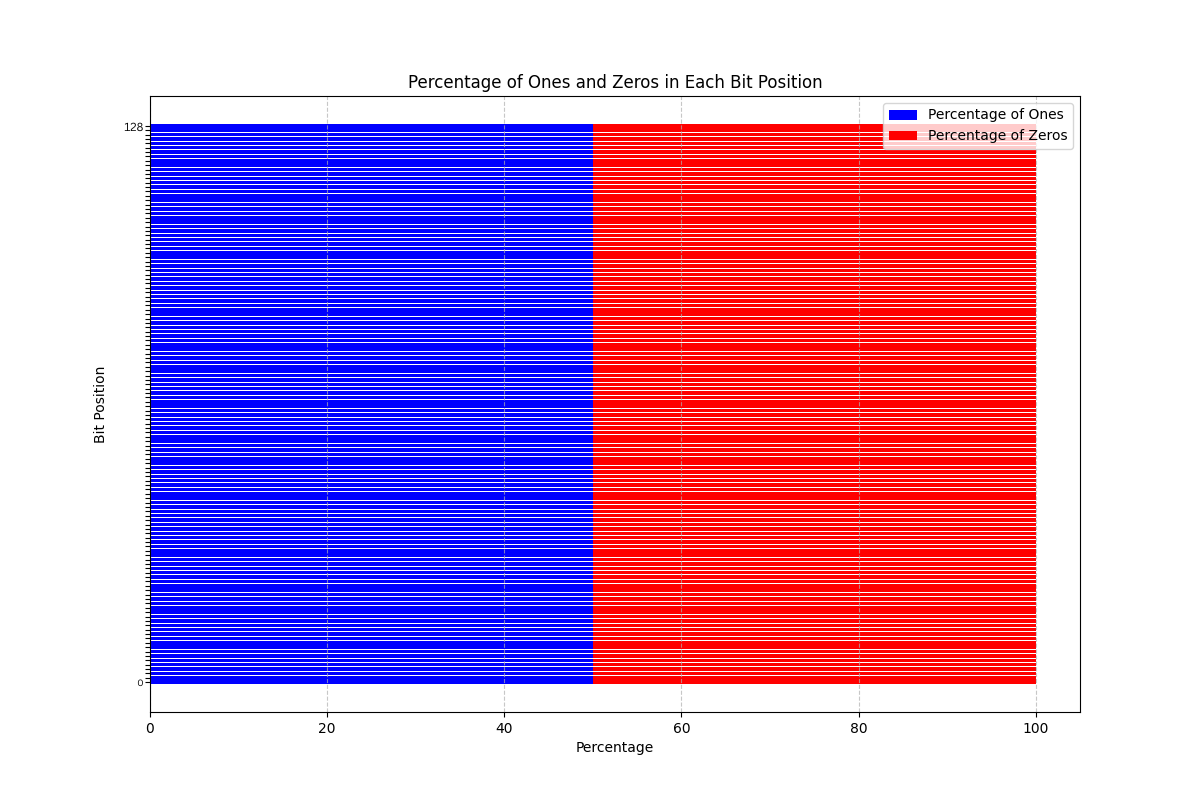
\includegraphics[width=1\textwidth]{final0s1sboth.png}
\caption{Plot of Counts for TEKs}
\label{fig:countsteks}
\end{figure}

\begin{figure}[H]
\centering
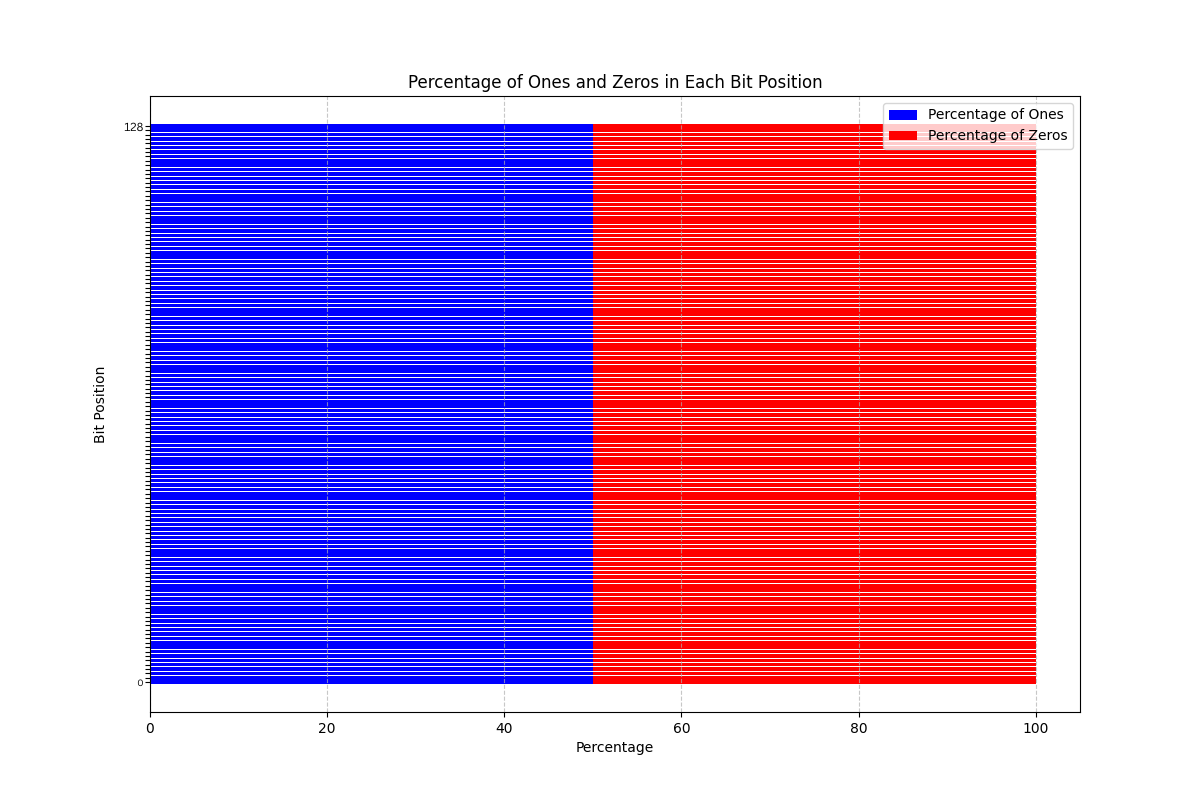
\includegraphics[width=1\textwidth]{final0s1sboth.png}
\caption{Plot of Counts for random keys}
\label{fig:countsrands}
\end{figure}

\subsection{Hilbert Curve}

The Hilbert Curve of the TEKs can be seen in Figure \ref{fig:hilbertteks} and the Hilbert Curve of the random keys can be seen in Figure \ref{fig:hilbertrands}. The Hilbert curve produced from both datasets are very similar and both show no evidence of non randomness. A uniform pattern in the graph indicates that the data is randomly distributed. There is no clustering or high density areas within either graph that would indicate non randomness. 

\begin{figure}[H]
\centering
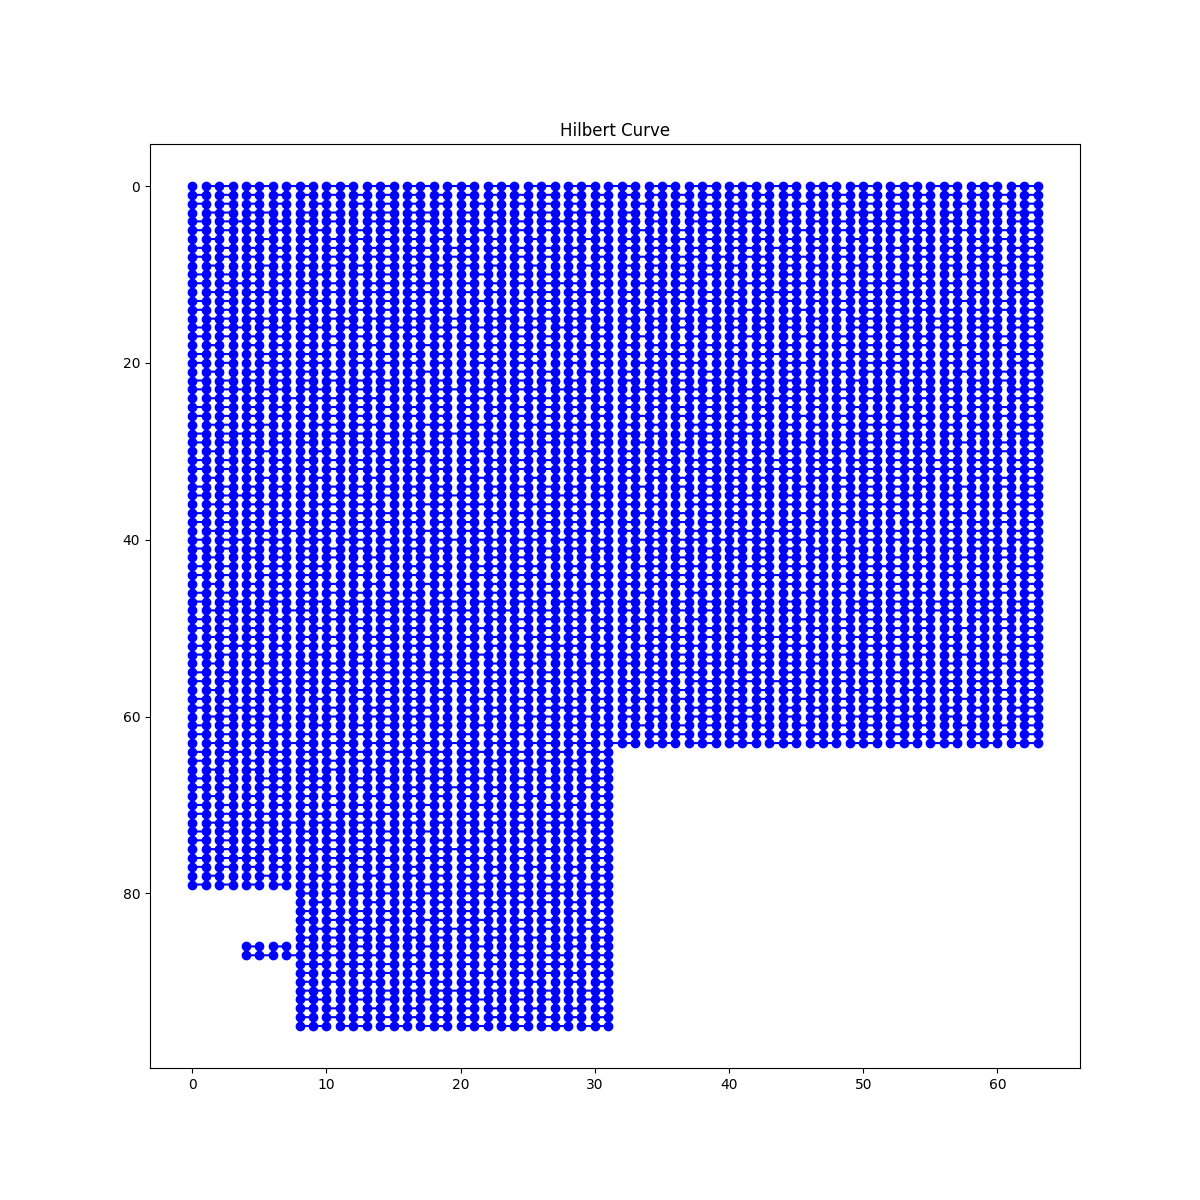
\includegraphics[width=1\textwidth]{hilbertCurveteks.png}
\caption{Hilbert Curve of TEKs}
\label{fig:hilbertteks}
\end{figure}

\begin{figure}[H]
\centering
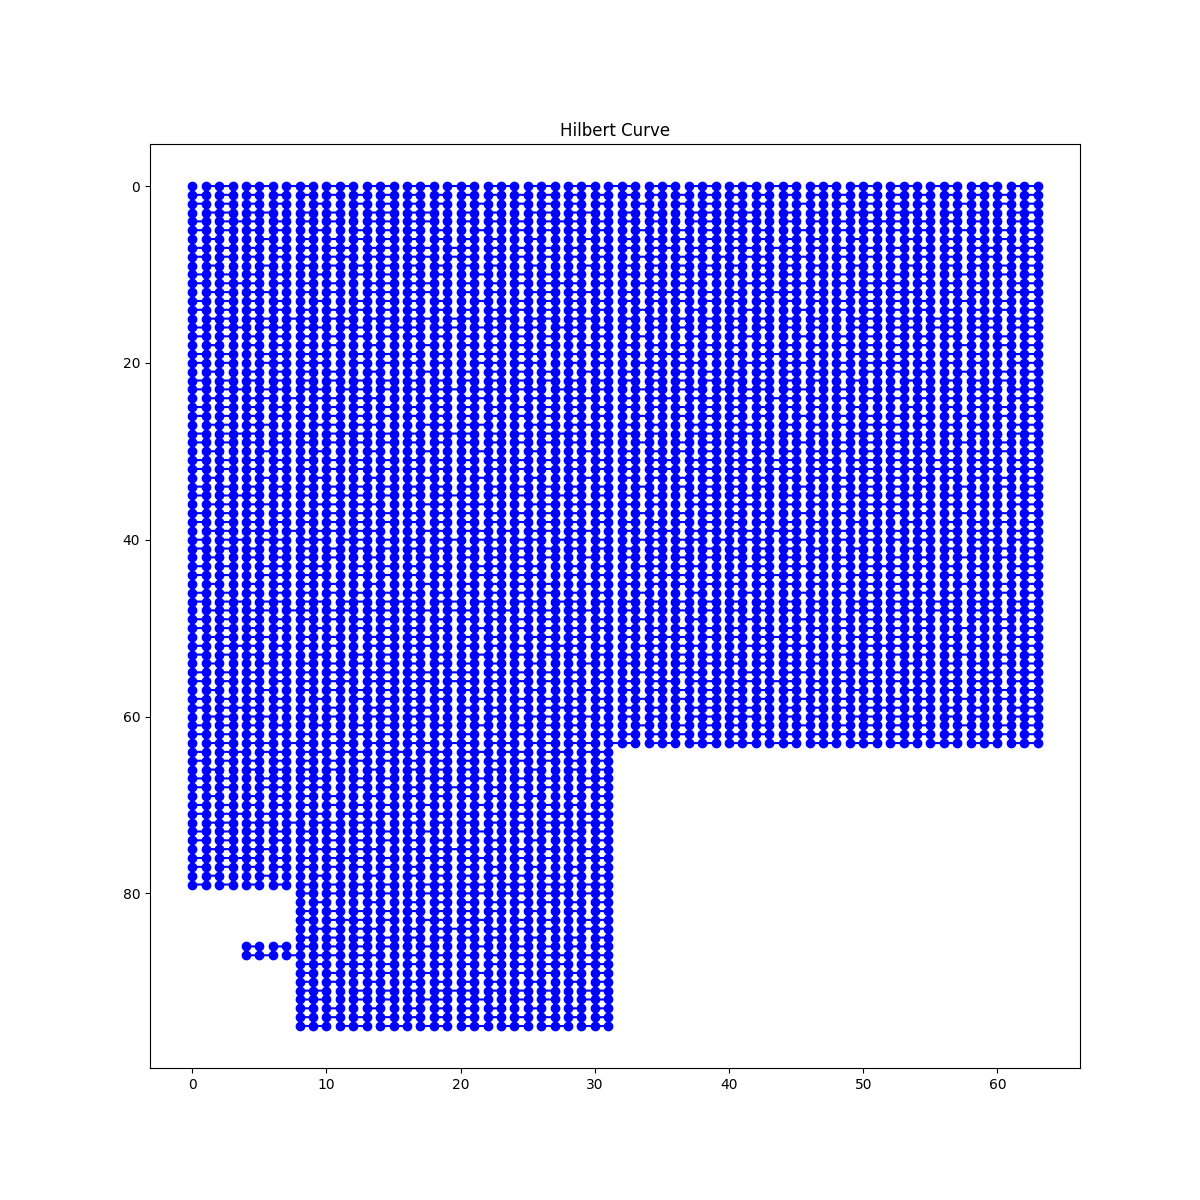
\includegraphics[width=1\textwidth]{hilbertCurverands.png}
\caption{Hilbert Curve of Random keys}
\label{fig:hilbertrands}
\end{figure}

\subsection{Lag Plot}


\begin{figure}[H]
\centering
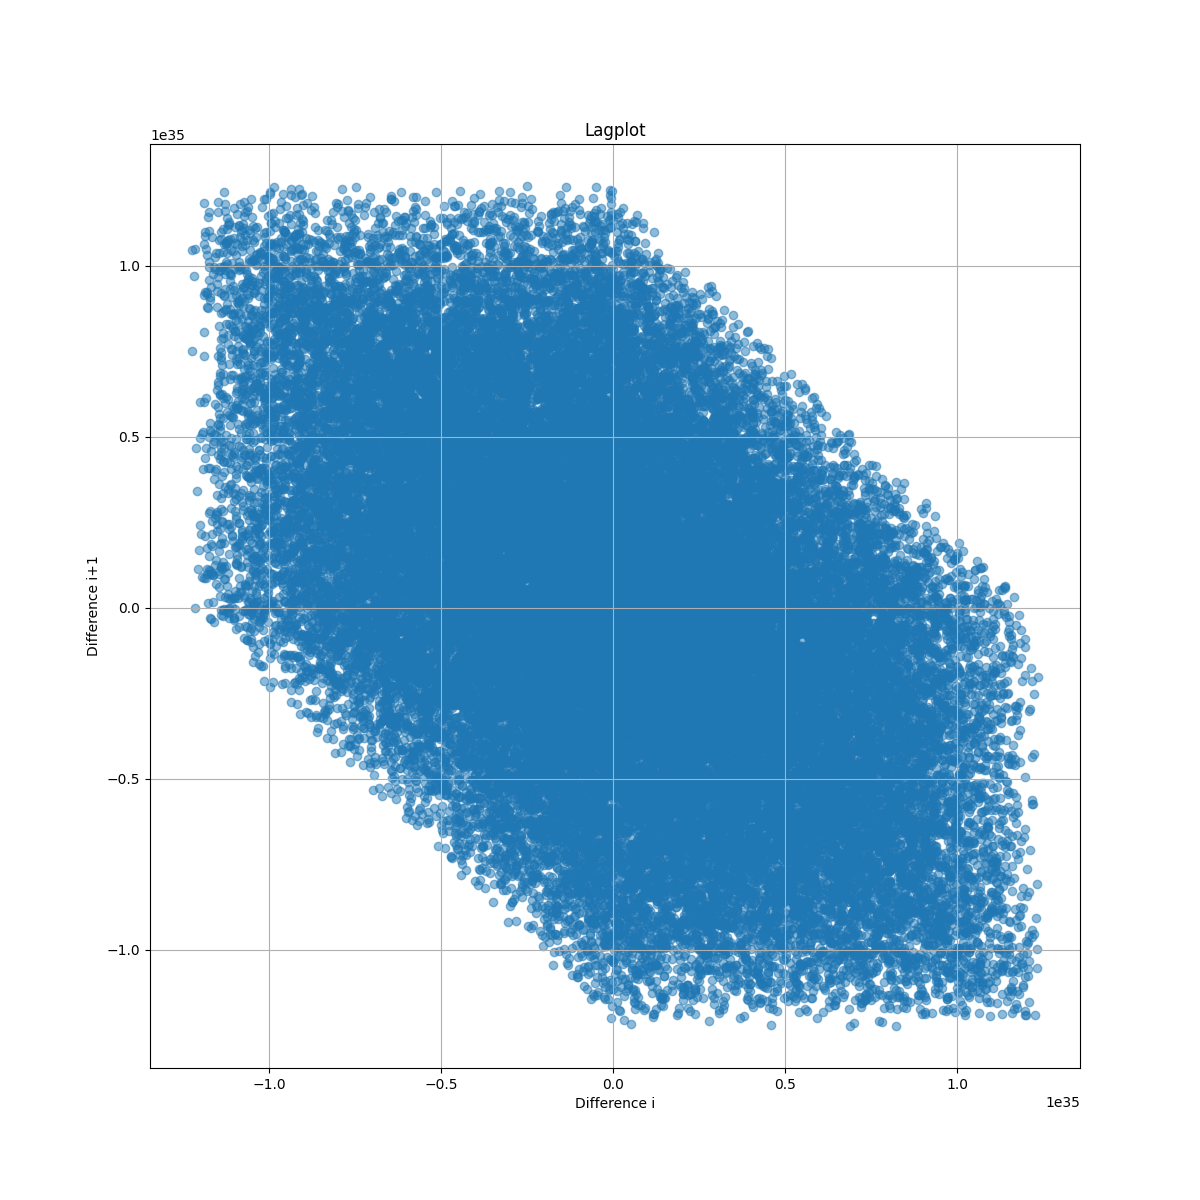
\includegraphics[width=1\textwidth]{lagplotteks50k.png}
\caption{Lag Plot of TEKs}
\label{fig:lagplotteks}
\end{figure}

\begin{figure}[H]
\centering
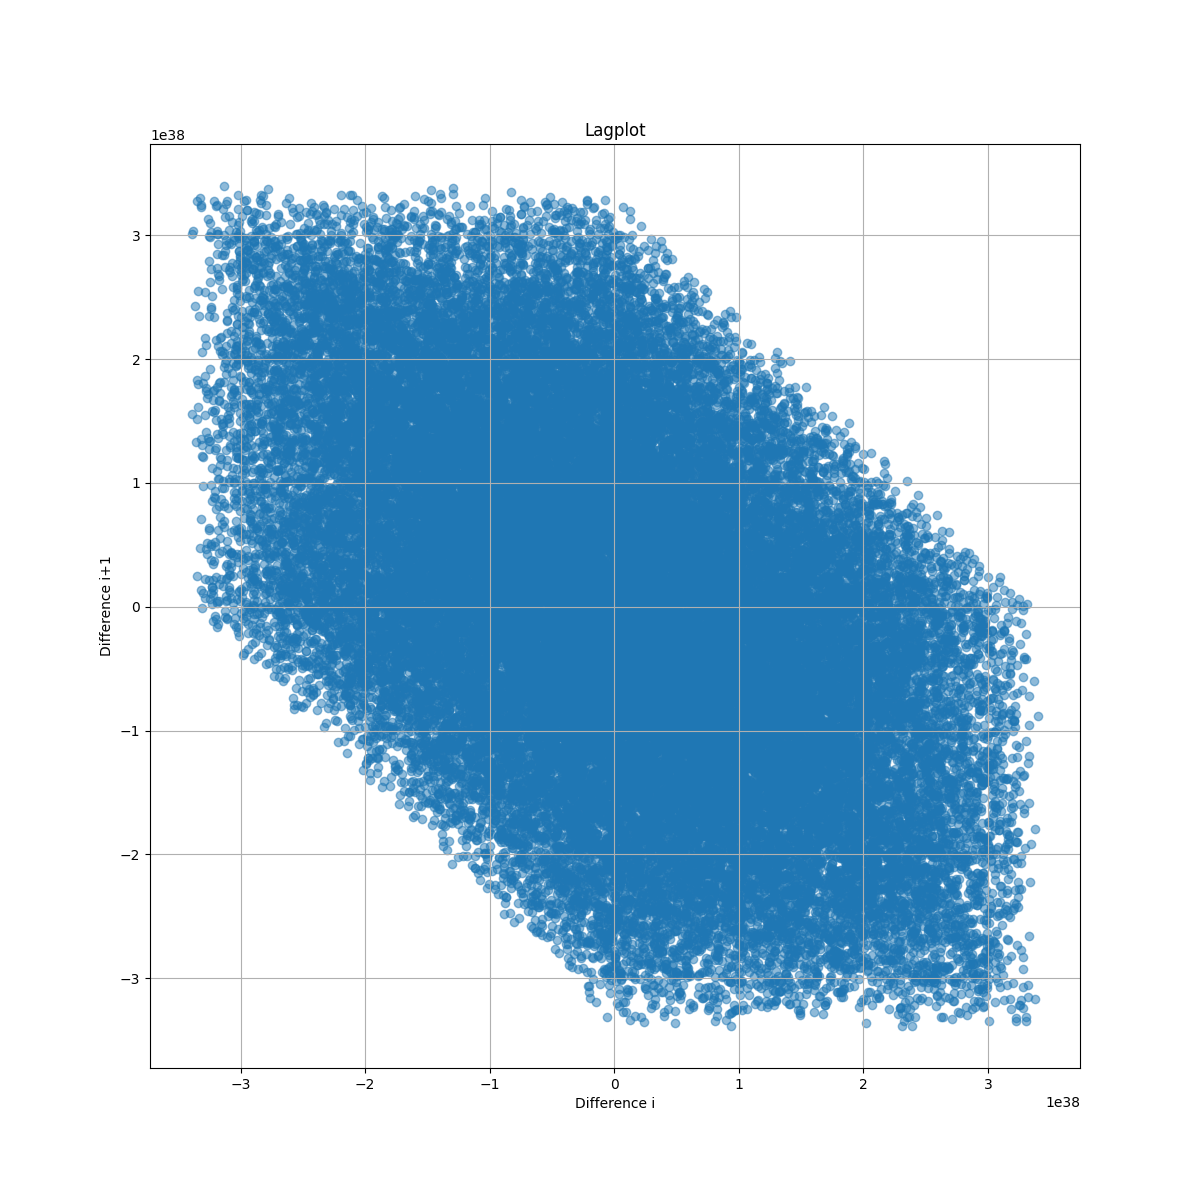
\includegraphics[width=1\textwidth]{lagplotrands50k.png}
\caption{Lag Plot of Random keys}
\label{fig:lagplotrands}
\end{figure}

\subsection{Chi-squared Test}

\begin{table}[H]
\centering
\begin{tabular}{|l|l|l|}
\cline{1-3}
\textbf{Dataset} & \textbf{Chi-squared Statistic}        & \textbf{P-value} \\ \cline{1-3}
TEKs             & 0.4601405325882503  & 0.49755830241590926     \\ \cline{1-3}
Random keys      & 0.6229208548153906 &   0.42996394455596043    \\ \cline{1-3}
\end{tabular}
\caption{Chi-squared Test Result}
\label{table}
\end{table}

\subsection{Spectral Test}

\begin{table}[H]
\centering
\begin{tabular}{|l|l|l|l|}
\cline{1-4}
\textbf{Dataset} & \textbf{no. rejected}        & \textbf{total} & \textbf{Percentage \%}\\ \cline{1-4}
TEKs             & 6080630  & 137358786    & 4.426822758902368 \\ \cline{1-4}
Random keys      & 7501794 &   169541632   &  4.424750376355938 \\ \cline{1-4}
\end{tabular}
\caption{Spectral Test Result}
\label{table}
\end{table}

\section{Conclusions}